\chapter*{Results}
\label{chap:Results}
\setcounter{section}{0}

During my thesis i learnt a lot about posture and sensors and achieved a great base for further projects and continuing this journey. I definitely did not create a finished product, however this was never the goal of this projects. Non the less i achieved a view goals which I have listed below.

\section{Quick Summary}

As a quick summary of all goals and learning, it can be said, that a minimum of two Sensors are needed from which one must be positioned on the lower back and one on the upper back. Due to this positioning it is nearly impossible to change posutre without the sensors to detect it. Additional sensor would help improving precision and fine tuning however are not necessary. The right posture is defined by the user itself and not defined by the software. A "global" correct position could be set using this setup, however was found not to be useful or recommendable. \cite{SitUpSt77:online} Additionally the user can also set posture he would like to avoid.

The user gets a vibration feedback from the sensor, and a visual feedback from the software when the set posture goal is not met. The analysis of these value is done with the median of a 10 second measurement, since a quicker refresh rate does not offer any real benefit and it reduces useless vibrations due to hectic movement.

\section{Achieved Goals}

In the evolution of this project. I simplified the data transfer and created a first definition how the sensors can be "dumb". Thanks to this the "sensor packets" got much simpler and need much less soldering. I was able to move all logic from the devices to any language or system desired without losing any significant response time. 

\begin{figure}[h]
  \begin{center}
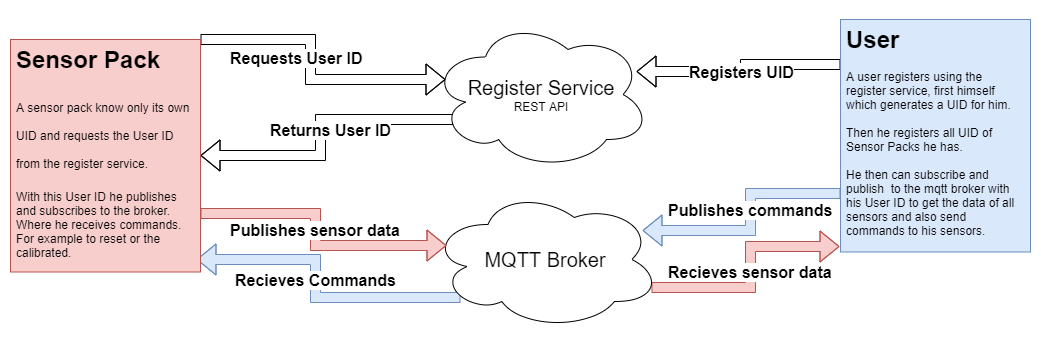
\includegraphics[width=\textwidth]{images/DumbSensor.png}
  \end{center}
  \caption{Sensor workflow}
  \label{fig:SensorWorkflow}
\end{figure}

With the flow displayed above (\ref{fig:SensorWorkflow}) the sensors can all have the same logic and only need  a unique id to be identified and no further setup. It needs to be noted, that the register service was not fully implemented for this thesis, however it was mocked. This since it does not add any value to the thesis or the goals of this thesis.

Thanks to these adjustments and improvements during this project, live data visualisation was achieved. This is on one hand a cool feature however it also simplifies the analysis and understanding of the collected data vastly. It helped me really understand the data and transfer it to a simple posture model. Which then enabled me to visualise the positioning of the sensors and the posture. Additionally thanks to my better understanding of the sensor data and collected data, how it can be used to model posture and my experience gained through the first versions, I know how a single self contained sensor pack could be implemented. This would be easier to user however much more restricted. 

Also due to the abstraction of logic, it became much easier working with the data and I think it also improved the re-usability, since logic can be implemented in any language desired and is not restricted to c++.

\subsection{Improving Posture}

Posture is quite a difficult topic, and I would be overselling, when writing, that I can improve posture with this concept. Since I have not many long term tests or studies I cannot confirm or deny that. However what I can do is read about good posture and how it can be improved and try to follow these principals. This is exactly what I did. According to the paper ""Sit Up Straight": Time to Re-evaluate" \cite{SitUpSt77:online} the right posture is not globally given or can be set for every person on this planet. 

In the following graphics the writer of the paper summarised their findings:
\begin{figure}[h]
  \begin{center}
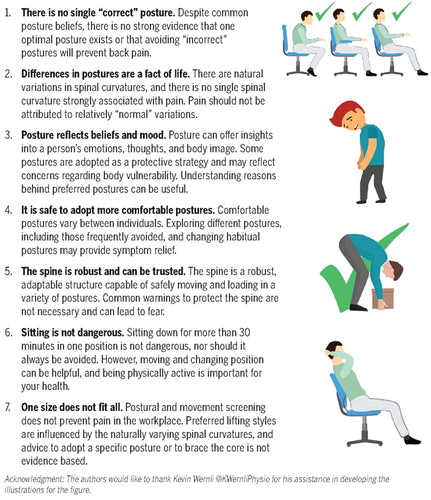
\includegraphics[width=0.5\textwidth]{images/jospt-562-fig001.jpg}
  \end{center}
  \caption{Posture Study}
  \label{fig:Posture Study}
\end{figure}

Most interesting for me are the first two points, which indicate that my posture module must be agile and adjustable to each user individually. This is also why i did not set a default goal, which a user must try to achieve. Each user can set their own goals. According to my understanding, it is the only way to safely and individually improve posture.This approach still has some risks and might lead to uncertainties with users. 
The user might not know what a good posture is and train a wrong posture or be afraid of training a wrong posture and not using this concept. This could be tackled by contacting a professional for a first input and an initial setup of the device.

\subsection{Being Open source}

All the code created for this project will be released on my git repository soon. An introduction and explanation will be available as well, including a list of parts needed to build the same devices. The code and all the documentation will be available as soon, as the code has reached a standard and cleanliness I can get behind. The Goal is to accomplish this at the time of submitting this paper.

\section{Open Goals}

From my goal of creating a simple affordable solution to improve posture, a lot has been achieved. Nonetheless I did not create the type of solution I first had in mind. I would not consider this a problem, since the current solution is much more flexible. However my first goal, which i tried to achieve in the first version, was a single contained unit which achieves posture improvements. This would be possible with the know-how i have now and will also be kept as a long term goal. However i feel that much more can be achieved with the distributed network i have implemented currently. 

Currently this sensor network is a simple proof of concept and I will definitely need to implemented some things I have mocked to create a usable and user friendly product.  The Register service would need to be implmented and also the web app needs a lot more work. It is currently not very user friendly and only configured to work with my 3 sensors. 

Furthermore when the register service is available the sensors need more work, to enable a complete self provisioning, since currently the network connection is hard coded. This is not very interesting or hard since it has been implemented multiple times (https://www.arduino.cc/en/Reference/WiFiNINABeginProvision), therefore i left it out. 

Security also is an issue that was only thought of however not implemented correctly. Currently the MQTT Broker is a secured by credentials however these also are hard-coded and would need to be different for every user. MQTT offers this possibility and also encrypts the messages.

Lastly the size of the sensor packets is far from optimal and could be drastically reduced by creating a single plate with all logic withing. This will not be a goal that I will tackles soon, since this would be the last step of creating such a "product".

\section{Similar Products}

\subsection{sming}

\begin{wrapfigure}{R}{0.15\textwidth}
  \begin{center}
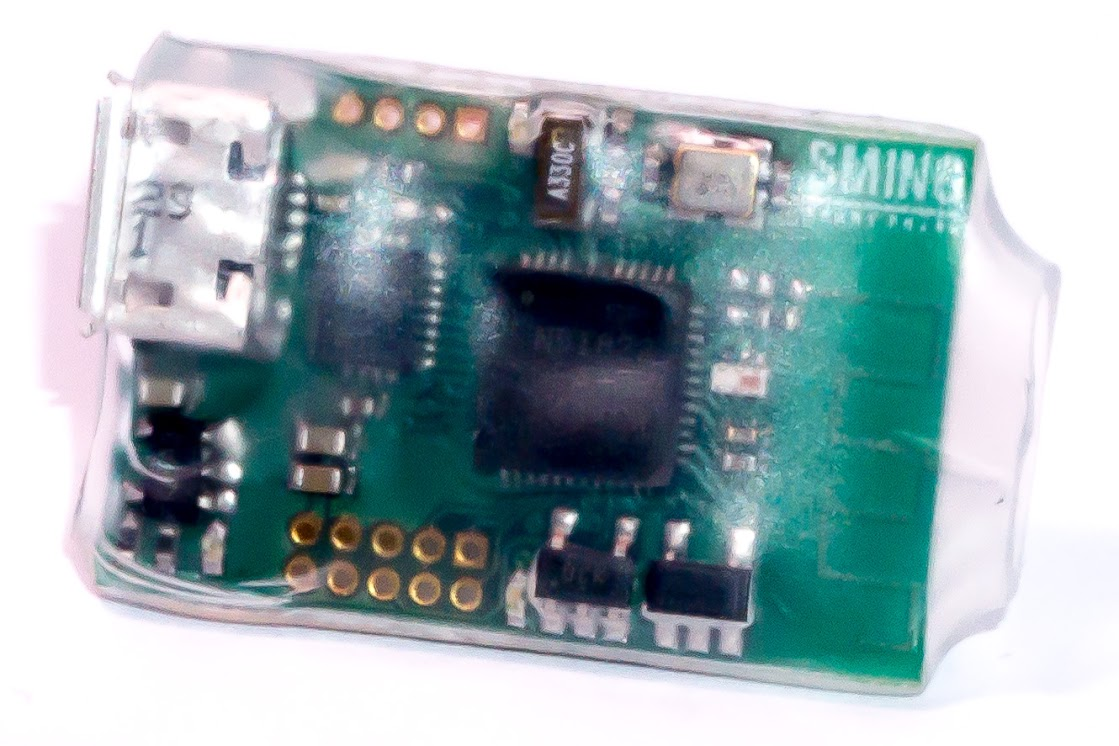
\includegraphics[width=\linewidth]{images/sming_pic2.jpg}
  \end{center}
  \caption{\label{fig:Sming}Sming}
\end{wrapfigure}
A Very important part of any "new" product is investigating what already exists on the market.
Usually someone already had a similar idea, or something which tries to solve the same problems has already been produced. 

The first similar product i would like to name is the "SMING" which is a sensor node created with the BFH. 
It is using the Sensor "TXW51" which has an acceleromter and a gyroscope. This devices uses Bluetooth smart to communicate. It was created for a master thesis and is a great example of how small such a device can be. 

It was planned to use the device for sports measurement and was designed to very energy efficient. However according to my know-how the device never has been in use productively. \cite{sming:book}
Such a device and the know-how gathered for this projects might be a great starting point when designing a "all in one" sensor packet for my use case. "SMING" might offer a lot even when used as is. This will need to be evaluated in the near future.

\subsection{Swaystar}

\begin{wrapfigure}{R}{0.15\textwidth}
  \begin{center}
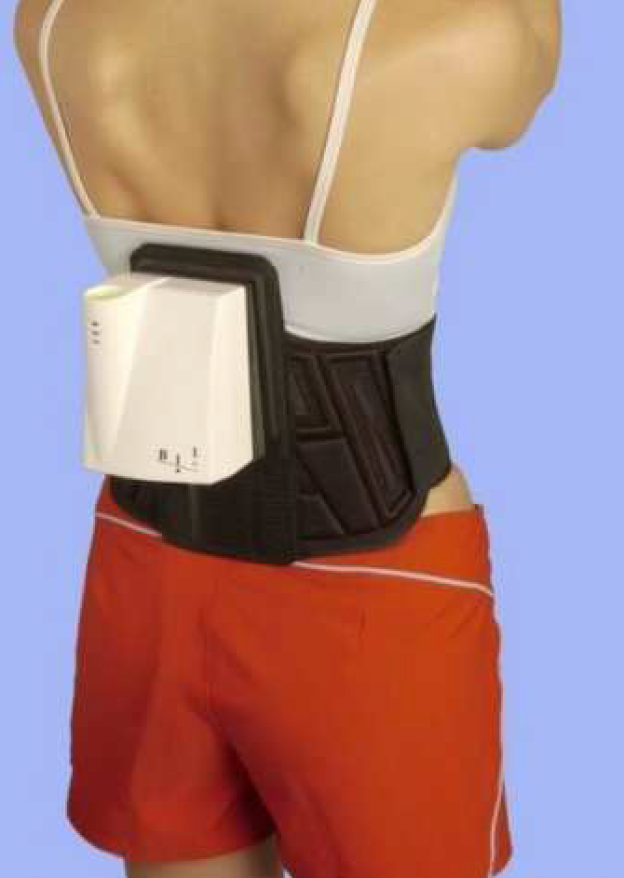
\includegraphics[width=\linewidth]{images/Swaystar_01.png}
  \end{center}
  \caption{\label{fig:swaystar}Swaystar}
\end{wrapfigure}

The following existing product was the trigger for my project idea. The so called swaystar \ref{fig:swaystar} offers almost the same functionality, however it is at least 10 times bigger and costs about 10'000 CHF. 
I have never used such a device, however i have talked to people who worked with one. Apparently it tracks the movement / positioning of users and stores the data. An additional headband can be purchased with which vibrations are sent to the user so he can improve his body ergonomics and balance. 

As said, it offers a very similar functionality, however not it covers the same use cases. Due to the size and price it can almost exclusively only be used in therapies and by medical professionals. My device intends to target the end user, and offer an easier and more affordable solution. The swaystar also is closed-source and appears to be a rather old product.
\cite{SwayStar47:online}

\newpage

\begin{wrapfigure}{r}{0.2\textwidth}
  \begin{center}
  \vspace{-20pt}
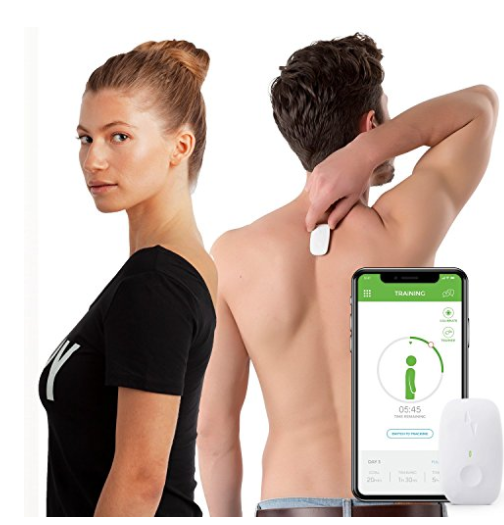
\includegraphics[width=\linewidth]{images/Screenshot_3.png}
  \end{center}
  \vspace{-10pt}
  \caption{Go Posture trainer}
  \label{fig:gotrainer}
  \vspace{-10pt}
\end{wrapfigure}

\subsection{Go Posture trainer}

Further investigations into other products, were almost fruitless. There are some apps which offer almost the same thing I have tried to achieve with my app, but a bit more refined and there is one product which offers a use-case that could be considered equal to the first defined use-case (improved sitting posture), at least on first glance (\ref{fig:gotrainer} Go Trainer). 

The product functions as a posture trainer, however it has to be attached to the back, and it is, even if small, quite visible under a shirt. Secondly the device only offers a mono-directional biofeedback. \cite{HowToImp2:online}

Furthermore the device is closed source and is only targeted to users who want to improve their posture. As mentioned the plan for my device would be to keep everything open-source and cover a wider range of use-cases. 

Most other devices to improve posture use cloth to physically "pull" the user in the right position.

After all these investigations and also further investigations into the medical field I considered my device to still be an innovation, offering something which is not yet available on the market.


\section{Learnings}

Firstly I understood how the MPU6050 sensor works with the wire library, learned much more about Arduino coding. I also learned the communication with other sensors and actors, like the SD card reader or the real time clock. Furthermore I learned what to be aware of when working with micro-controllers, how to setup a simple client server network with minimal resources. All of this was necessary to achieve a simplified and usable sensor pack. 
To position the sensor pack i had to test multiple positioning and discuss with a physiotherapist what a useful position would be. According to my understanding the current optimal position would be directly on the spine, and at least two sensors, one on the upper and one on the lower back. Every additional sensor improves the precision of the posture model. 

Additionally the learning will be applicable on the first version of the project. As mentioned two sensors are necessary for a useful analysis of posture, nonetheless with the current know-how I know that some measurements are still possible with a single sensor unit. it will need to be analysed with a long-term test, how much information is lost when using a single sensor and whether the lost information is critical for a daily wearer.

To understand the positioning I also had to understand what posture is. This was only possible through research and unfortunately this know how is still very limited.

\section{Project Management}

In the beginning of the Project a lot of goals were defined. These goals were tagged as necessary or optional. However the goals changed greatly during the thesis, since new ideas emerged. Non-theless the primary necessary goals, stayed the same and are defined as follows: 

\begin{center}
\begin{table}[h!]
\begin{tabular}{|p{9cm}|p{3cm}|p{3cm}|}
  \hline
 \textbf{Goal} &\textbf{ Planned  } &\textbf{ Completed By } \\ 
  \hline
 Communication between ESP32 and Sensors & July 2019 & July 2019   \\  
 \hline
 Collect the data  & August 2019  & August 2019   \\  
  \hline
 Enable multi Sensor communication (Client, Server) & September 2019 & September 2019   \\ 
  \hline
 Enable multi Sensor communication (MQTT) & - & October 2019   \\ 
  \hline
 Visualise the data & October 2019 & November 2019   \\  
  \hline
 Real time visualisation (WebApp) & - & December 2019   \\  
   \hline
 Sensor position and amount & November 2019 & December 2019   \\ 
  \hline
 Identify posture & November 2019 & December 2019   \\  
  \hline
 Visualise posture & December 2019 &  December 2019 \\    
   \hline
 Visualise and communicate wrong posture & December 2019& January 2020 \\    
  \hline~
\end{tabular}
\caption{Planned and unplanned goals}
\label{table:1}
\end{table}
\end{center}

\subsection{Technical implementation later than expected}

Originally it was planned to have everything technical, software and hardware, done in the beginning of December. However due to the MQTT data transfer implementation and the visualisation of the data with a web app a lot of the work got done later than expected. However this was manageable since a time buffer was planned in the beginning. Three weeks of holidays in December were planned in the beginning of the project to ensure a certain and non-hectical finish of the implementation. As visible in the table, this three weeks were used and were definitely necessary. 
